\documentclass[1p]{elsarticle_modified}
%\bibliographystyle{elsarticle-num}

%\usepackage[colorlinks]{hyperref}
%\usepackage{abbrmath_seonhwa} %\Abb, \Ascr, \Acal ,\Abf, \Afrak
\usepackage{amsfonts}
\usepackage{amssymb}
\usepackage{amsmath}
\usepackage{amsthm}
\usepackage{scalefnt}
\usepackage{amsbsy}
\usepackage{kotex}
\usepackage{caption}
\usepackage{subfig}
\usepackage{color}
\usepackage{graphicx}
\usepackage{xcolor} %% white, black, red, green, blue, cyan, magenta, yellow
\usepackage{float}
\usepackage{setspace}
\usepackage{hyperref}

\usepackage{tikz}
\usetikzlibrary{arrows}

\usepackage{multirow}
\usepackage{array} % fixed length table
\usepackage{hhline}

%%%%%%%%%%%%%%%%%%%%%
\makeatletter
\renewcommand*\env@matrix[1][\arraystretch]{%
	\edef\arraystretch{#1}%
	\hskip -\arraycolsep
	\let\@ifnextchar\new@ifnextchar
	\array{*\c@MaxMatrixCols c}}
\makeatother %https://tex.stackexchange.com/questions/14071/how-can-i-increase-the-line-spacing-in-a-matrix
%%%%%%%%%%%%%%%

\usepackage[normalem]{ulem}

\newcommand{\msout}[1]{\ifmmode\text{\sout{\ensuremath{#1}}}\else\sout{#1}\fi}
%SOURCE: \msout is \stkout macro in https://tex.stackexchange.com/questions/20609/strikeout-in-math-mode

\newcommand{\cancel}[1]{
	\ifmmode
	{\color{red}\msout{#1}}
	\else
	{\color{red}\sout{#1}}
	\fi
}

\newcommand{\add}[1]{
	{\color{blue}\uwave{#1}}
}

\newcommand{\replace}[2]{
	\ifmmode
	{\color{red}\msout{#1}}{\color{blue}\uwave{#2}}
	\else
	{\color{red}\sout{#1}}{\color{blue}\uwave{#2}}
	\fi
}

\newcommand{\Sol}{\mathcal{S}} %segment
\newcommand{\D}{D} %diagram
\newcommand{\A}{\mathcal{A}} %arc


%%%%%%%%%%%%%%%%%%%%%%%%%%%%%5 test

\def\sl{\operatorname{\textup{SL}}(2,\Cbb)}
\def\psl{\operatorname{\textup{PSL}}(2,\Cbb)}
\def\quan{\mkern 1mu \triangleright \mkern 1mu}

\theoremstyle{definition}
\newtheorem{thm}{Theorem}[section]
\newtheorem{prop}[thm]{Proposition}
\newtheorem{lem}[thm]{Lemma}
\newtheorem{ques}[thm]{Question}
\newtheorem{cor}[thm]{Corollary}
\newtheorem{defn}[thm]{Definition}
\newtheorem{exam}[thm]{Example}
\newtheorem{rmk}[thm]{Remark}
\newtheorem{alg}[thm]{Algorithm}

\newcommand{\I}{\sqrt{-1}}
\begin{document}

%\begin{frontmatter}
%
%\title{Boundary parabolic representations of knots up to 8 crossings}
%
%%% Group authors per affiliation:
%\author{Yunhi Cho} 
%\address{Department of Mathematics, University of Seoul, Seoul, Korea}
%\ead{yhcho@uos.ac.kr}
%
%
%\author{Seonhwa Kim} %\fnref{s_kim}}
%\address{Center for Geometry and Physics, Institute for Basic Science, Pohang, 37673, Korea}
%\ead{ryeona17@ibs.re.kr}
%
%\author{Hyuk Kim}
%\address{Department of Mathematical Sciences, Seoul National University, Seoul 08826, Korea}
%\ead{hyukkim@snu.ac.kr}
%
%\author{Seokbeom Yoon}
%\address{Department of Mathematical Sciences, Seoul National University, Seoul, 08826,  Korea}
%\ead{sbyoon15@snu.ac.kr}
%
%\begin{abstract}
%We find all boundary parabolic representation of knots up to 8 crossings.
%
%\end{abstract}
%\begin{keyword}
%    \MSC[2010] 57M25 
%\end{keyword}
%
%\end{frontmatter}

%\linenumbers
%\tableofcontents
%
\newcommand\colored[1]{\textcolor{white}{\rule[-0.35ex]{0.8em}{1.4ex}}\kern-0.8em\color{red} #1}%
%\newcommand\colored[1]{\textcolor{white}{ #1}\kern-2.17ex	\textcolor{white}{ #1}\kern-1.81ex	\textcolor{white}{ #1}\kern-2.15ex\color{red}#1	}

{\Large $\underline{12n_{0521}~(K12n_{0521})}$}

\setlength{\tabcolsep}{10pt}
\renewcommand{\arraystretch}{1.6}
\vspace{1cm}\begin{tabular}{m{100pt}>{\centering\arraybackslash}m{274pt}}
\multirow{5}{120pt}{
	\centering
	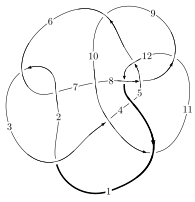
\includegraphics[width=112pt]{../../../GIT/diagram.site/Diagrams/png/2610_12n_0521.png}\\
\ \ \ A knot diagram\footnotemark}&
\allowdisplaybreaks
\textbf{Linearized knot diagam} \\
\cline{2-2}
 &
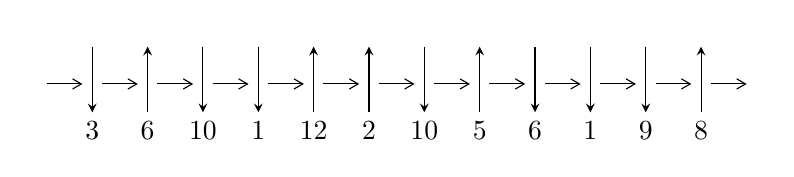
\begin{tikzpicture}[x=20pt, y=17pt]
	% nodes
	\node (C0) at (0, 0) {};
	\node (C1) at (1, 0) {};
	\node (C1U) at (1, +1) {};
	\node (C1D) at (1, -1) {3};

	\node (C2) at (2, 0) {};
	\node (C2U) at (2, +1) {};
	\node (C2D) at (2, -1) {6};

	\node (C3) at (3, 0) {};
	\node (C3U) at (3, +1) {};
	\node (C3D) at (3, -1) {10};

	\node (C4) at (4, 0) {};
	\node (C4U) at (4, +1) {};
	\node (C4D) at (4, -1) {1};

	\node (C5) at (5, 0) {};
	\node (C5U) at (5, +1) {};
	\node (C5D) at (5, -1) {12};

	\node (C6) at (6, 0) {};
	\node (C6U) at (6, +1) {};
	\node (C6D) at (6, -1) {2};

	\node (C7) at (7, 0) {};
	\node (C7U) at (7, +1) {};
	\node (C7D) at (7, -1) {10};

	\node (C8) at (8, 0) {};
	\node (C8U) at (8, +1) {};
	\node (C8D) at (8, -1) {5};

	\node (C9) at (9, 0) {};
	\node (C9U) at (9, +1) {};
	\node (C9D) at (9, -1) {6};

	\node (C10) at (10, 0) {};
	\node (C10U) at (10, +1) {};
	\node (C10D) at (10, -1) {1};

	\node (C11) at (11, 0) {};
	\node (C11U) at (11, +1) {};
	\node (C11D) at (11, -1) {9};

	\node (C12) at (12, 0) {};
	\node (C12U) at (12, +1) {};
	\node (C12D) at (12, -1) {8};
	\node (C13) at (13, 0) {};

	% arrows
	\draw[->,>={angle 60}]
	(C0) edge (C1) (C1) edge (C2) (C2) edge (C3) (C3) edge (C4) (C4) edge (C5) (C5) edge (C6) (C6) edge (C7) (C7) edge (C8) (C8) edge (C9) (C9) edge (C10) (C10) edge (C11) (C11) edge (C12) (C12) edge (C13) ;	\draw[->,>=stealth]
	(C1U) edge (C1D) (C2D) edge (C2U) (C3U) edge (C3D) (C4U) edge (C4D) (C5D) edge (C5U) (C6D) edge (C6U) (C7U) edge (C7D) (C8D) edge (C8U) (C9U) edge (C9D) (C10U) edge (C10D) (C11U) edge (C11D) (C12D) edge (C12U) ;
	\end{tikzpicture} \\
\hhline{~~} \\& 
\textbf{Solving Sequence} \\ \cline{2-2} 
 &
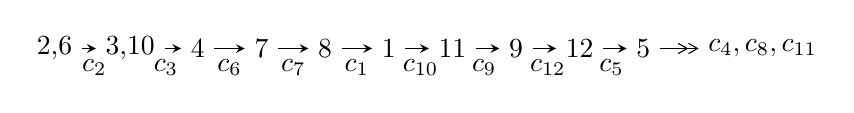
\begin{tikzpicture}[x=23pt, y=7pt]
	% node
	\node (A0) at (-1/8, 0) {2,6};
	\node (A1) at (17/16, 0) {3,10};
	\node (A2) at (17/8, 0) {4};
	\node (A3) at (25/8, 0) {7};
	\node (A4) at (33/8, 0) {8};
	\node (A5) at (41/8, 0) {1};
	\node (A6) at (49/8, 0) {11};
	\node (A7) at (57/8, 0) {9};
	\node (A8) at (65/8, 0) {12};
	\node (A9) at (73/8, 0) {5};
	\node (C1) at (1/2, -1) {$c_{2}$};
	\node (C2) at (13/8, -1) {$c_{3}$};
	\node (C3) at (21/8, -1) {$c_{6}$};
	\node (C4) at (29/8, -1) {$c_{7}$};
	\node (C5) at (37/8, -1) {$c_{1}$};
	\node (C6) at (45/8, -1) {$c_{10}$};
	\node (C7) at (53/8, -1) {$c_{9}$};
	\node (C8) at (61/8, -1) {$c_{12}$};
	\node (C9) at (69/8, -1) {$c_{5}$};
	\node (A10) at (11, 0) {$c_{4},c_{8},c_{11}$};

	% edge
	\draw[->,>=stealth]	
	(A0) edge (A1) (A1) edge (A2) (A2) edge (A3) (A3) edge (A4) (A4) edge (A5) (A5) edge (A6) (A6) edge (A7) (A7) edge (A8) (A8) edge (A9) ;
	\draw[->>,>={angle 60}]	
	(A9) edge (A10);
\end{tikzpicture} \\ 

\end{tabular} \\

\footnotetext{
The image of knot diagram is generated by the software ``\textbf{Draw programme}" developed by Andrew Bartholomew(\url{http://www.layer8.co.uk/maths/draw/index.htm\#Running-draw}), where we modified some parts for our purpose(\url{https://github.com/CATsTAILs/LinksPainter}).
}\phantom \\ \newline 
\centering \textbf{Ideals for irreducible components\footnotemark of $X_{\text{par}}$} 
 
\begin{align*}
I^u_{1}&=\langle 
432917 u^{27}+3841573 u^{26}+\cdots+262964 b+2783376,\\
\phantom{I^u_{1}}&\phantom{= \langle  }413130 u^{27}+3479001 u^{26}+\cdots+262964 a+1217429,\;u^{28}+9 u^{27}+\cdots+124 u+16\rangle \\
I^u_{2}&=\langle 
-87 u^{16}+385 u^{15}+\cdots+77 b-41,\;-190 u^{16}+693 u^{15}+\cdots+231 a-163,\;u^{17}-4 u^{16}+\cdots-6 u^2-1\rangle \\
I^u_{3}&=\langle 
343 u^{10} a^3+5345 u^{10} a^2+\cdots+5127 a+18129,\;u^{10} a^3-3 u^{10} a^2+\cdots+26 a+1,\\
\phantom{I^u_{3}}&\phantom{= \langle  }u^{11}-2 u^{10}+6 u^9-8 u^8+12 u^7-13 u^6+12 u^5-13 u^4+9 u^3-8 u^2+4 u-1\rangle \\
I^u_{4}&=\langle 
b- a+u,\;a^2+a- u-1,\;u^2+u+1\rangle \\
I^u_{5}&=\langle 
b- a+1,\;a^2- a u- a+1,\;u^2+u+1\rangle \\
\\
\end{align*}
\raggedright * 5 irreducible components of $\dim_{\mathbb{C}}=0$, with total 97 representations.\\
\footnotetext{All coefficients of polynomials are rational numbers. But the coefficients are sometimes approximated in decimal forms when there is not enough margin.}
\newpage
\renewcommand{\arraystretch}{1}
\centering \section*{I. $I^u_{1}= \langle 4.33\times10^{5} u^{27}+3.84\times10^{6} u^{26}+\cdots+2.63\times10^{5} b+2.78\times10^{6},\;4.13\times10^{5} u^{27}+3.48\times10^{6} u^{26}+\cdots+2.63\times10^{5} a+1.22\times10^{6},\;u^{28}+9 u^{27}+\cdots+124 u+16 \rangle$}
\flushleft \textbf{(i) Arc colorings}\\
\begin{tabular}{m{7pt} m{180pt} m{7pt} m{180pt} }
\flushright $a_{2}=$&$\begin{pmatrix}1\\0\end{pmatrix}$ \\
\flushright $a_{6}=$&$\begin{pmatrix}0\\u\end{pmatrix}$ \\
\flushright $a_{3}=$&$\begin{pmatrix}1\\- u^2\end{pmatrix}$ \\
\flushright $a_{10}=$&$\begin{pmatrix}-1.57105 u^{27}-13.2300 u^{26}+\cdots-55.0012 u-4.62964\\-1.64630 u^{27}-14.6087 u^{26}+\cdots-102.538 u-10.5846\end{pmatrix}$ \\
\flushright $a_{4}=$&$\begin{pmatrix}0.956809 u^{27}+9.01001 u^{26}+\cdots+2.45249 u-3.84208\\1.67232 u^{27}+15.4625 u^{26}+\cdots+188.238 u+21.6886\end{pmatrix}$ \\
\flushright $a_{7}=$&$\begin{pmatrix}u\\u\end{pmatrix}$ \\
\flushright $a_{8}=$&$\begin{pmatrix}-0.715515 u^{27}-6.45245 u^{26}+\cdots-184.785 u-26.5307\\0.687566 u^{27}+5.41127 u^{26}+\cdots-74.2301 u-11.6532\end{pmatrix}$ \\
\flushright $a_{1}=$&$\begin{pmatrix}u^2+1\\- u^4\end{pmatrix}$ \\
\flushright $a_{11}=$&$\begin{pmatrix}-0.693057 u^{27}-6.09592 u^{26}+\cdots+30.7434 u+7.11420\\-2.14571 u^{27}-18.5603 u^{26}+\cdots-94.5924 u-9.92361\end{pmatrix}$ \\
\flushright $a_{9}=$&$\begin{pmatrix}-1.57105 u^{27}-13.2300 u^{26}+\cdots-55.0012 u-4.62964\\-2.38308 u^{27}-20.2951 u^{26}+\cdots-14.8953 u+3.96757\end{pmatrix}$ \\
\flushright $a_{12}=$&$\begin{pmatrix}-1.33446 u^{27}-10.2494 u^{26}+\cdots-6.34518 u+1.73776\\1.02850 u^{27}+9.08118 u^{26}+\cdots+212.265 u+31.6255\end{pmatrix}$ \\
\flushright $a_{5}=$&$\begin{pmatrix}2.39557 u^{27}+20.4749 u^{26}+\cdots+148.520 u+18.4022\\1.49590 u^{27}+15.8334 u^{26}+\cdots+111.117 u+8.74080\end{pmatrix}$\\&\end{tabular}
\flushleft \textbf{(ii) Obstruction class $= -1$}\\~\\
\flushleft \textbf{(iii) Cusp Shapes $= -\frac{394167}{65741} u^{27}-\frac{3195674}{65741} u^{26}+\cdots-\frac{10576918}{65741} u-\frac{485930}{65741}$}\\~\\
\newpage\renewcommand{\arraystretch}{1}
\flushleft \textbf{(iv) u-Polynomials at the component}\newline \\
\begin{tabular}{m{50pt}|m{274pt}}
Crossings & \hspace{64pt}u-Polynomials at each crossing \\
\hline $$\begin{aligned}c_{1}\end{aligned}$$&$\begin{aligned}
&u^{28}+17 u^{27}+\cdots+1360 u+256
\end{aligned}$\\
\hline $$\begin{aligned}c_{2},c_{6}\end{aligned}$$&$\begin{aligned}
&u^{28}-9 u^{27}+\cdots-124 u+16
\end{aligned}$\\
\hline $$\begin{aligned}c_{3},c_{9}\end{aligned}$$&$\begin{aligned}
&u^{28}+u^{27}+\cdots+u+1
\end{aligned}$\\
\hline $$\begin{aligned}c_{4}\end{aligned}$$&$\begin{aligned}
&u^{28}-2 u^{27}+\cdots-45 u+25
\end{aligned}$\\
\hline $$\begin{aligned}c_{5},c_{8}\end{aligned}$$&$\begin{aligned}
&u^{28}+u^{26}+\cdots+3 u+1
\end{aligned}$\\
\hline $$\begin{aligned}c_{7},c_{10}\end{aligned}$$&$\begin{aligned}
&u^{28}+u^{27}+\cdots+21 u+1
\end{aligned}$\\
\hline $$\begin{aligned}c_{11}\end{aligned}$$&$\begin{aligned}
&u^{28}-28 u^{27}+\cdots-50 u+4
\end{aligned}$\\
\hline $$\begin{aligned}c_{12}\end{aligned}$$&$\begin{aligned}
&u^{28}-26 u^{27}+\cdots-5120 u+512
\end{aligned}$\\
\hline
\end{tabular}\\~\\
\newpage\renewcommand{\arraystretch}{1}
\flushleft \textbf{(v) Riley Polynomials at the component}\newline \\
\begin{tabular}{m{50pt}|m{274pt}}
Crossings & \hspace{64pt}Riley Polynomials at each crossing \\
\hline $$\begin{aligned}c_{1}\end{aligned}$$&$\begin{aligned}
&y^{28}-11 y^{27}+\cdots+264448 y+65536
\end{aligned}$\\
\hline $$\begin{aligned}c_{2},c_{6}\end{aligned}$$&$\begin{aligned}
&y^{28}+17 y^{27}+\cdots+1360 y+256
\end{aligned}$\\
\hline $$\begin{aligned}c_{3},c_{9}\end{aligned}$$&$\begin{aligned}
&y^{28}-31 y^{27}+\cdots-7 y+1
\end{aligned}$\\
\hline $$\begin{aligned}c_{4}\end{aligned}$$&$\begin{aligned}
&y^{28}-16 y^{27}+\cdots-10575 y+625
\end{aligned}$\\
\hline $$\begin{aligned}c_{5},c_{8}\end{aligned}$$&$\begin{aligned}
&y^{28}+2 y^{27}+\cdots+y+1
\end{aligned}$\\
\hline $$\begin{aligned}c_{7},c_{10}\end{aligned}$$&$\begin{aligned}
&y^{28}-39 y^{27}+\cdots-197 y+1
\end{aligned}$\\
\hline $$\begin{aligned}c_{11}\end{aligned}$$&$\begin{aligned}
&y^{28}-22 y^{27}+\cdots-188 y+16
\end{aligned}$\\
\hline $$\begin{aligned}c_{12}\end{aligned}$$&$\begin{aligned}
&y^{28}-6 y^{27}+\cdots-1310720 y+262144
\end{aligned}$\\
\hline
\end{tabular}\\~\\
\newpage\flushleft \textbf{(vi) Complex Volumes and Cusp Shapes}
$$\begin{array}{c|c|c}  
\text{Solutions to }I^u_{1}& \I (\text{vol} + \sqrt{-1}CS) & \text{Cusp shape}\\
 \hline 
\begin{aligned}
u &= -0.029760 + 1.024060 I \\
a &= -0.76705 + 1.20618 I \\
b &= \phantom{-}0.33513 + 2.03849 I\end{aligned}
 & -1.70801 + 1.93955 I & -4.01504 - 3.31370 I \\ \hline\begin{aligned}
u &= -0.029760 - 1.024060 I \\
a &= -0.76705 - 1.20618 I \\
b &= \phantom{-}0.33513 - 2.03849 I\end{aligned}
 & -1.70801 - 1.93955 I & -4.01504 + 3.31370 I \\ \hline\begin{aligned}
u &= -0.205800 + 0.952470 I \\
a &= -0.890270 - 0.134444 I \\
b &= -1.028510 + 0.354995 I\end{aligned}
 & -1.87676 - 2.57239 I & -5.76873 + 3.90772 I \\ \hline\begin{aligned}
u &= -0.205800 - 0.952470 I \\
a &= -0.890270 + 0.134444 I \\
b &= -1.028510 - 0.354995 I\end{aligned}
 & -1.87676 + 2.57239 I & -5.76873 - 3.90772 I \\ \hline\begin{aligned}
u &= \phantom{-}0.703844 + 0.651022 I \\
a &= \phantom{-}0.364061 + 0.072255 I \\
b &= -0.169040 - 0.626677 I\end{aligned}
 & \phantom{-}2.58954 - 1.93444 I & \phantom{-}4.44360 + 1.82417 I \\ \hline\begin{aligned}
u &= \phantom{-}0.703844 - 0.651022 I \\
a &= \phantom{-}0.364061 - 0.072255 I \\
b &= -0.169040 + 0.626677 I\end{aligned}
 & \phantom{-}2.58954 + 1.93444 I & \phantom{-}4.44360 - 1.82417 I \\ \hline\begin{aligned}
u &= -0.233119 + 1.022850 I \\
a &= \phantom{-}0.432125 - 0.884732 I \\
b &= \phantom{-}0.046325 - 1.319720 I\end{aligned}
 & -0.84729 - 2.02401 I & -1.05491 + 4.41629 I \\ \hline\begin{aligned}
u &= -0.233119 - 1.022850 I \\
a &= \phantom{-}0.432125 + 0.884732 I \\
b &= \phantom{-}0.046325 + 1.319720 I\end{aligned}
 & -0.84729 + 2.02401 I & -1.05491 - 4.41629 I \\ \hline\begin{aligned}
u &= -0.592728 + 0.886067 I \\
a &= \phantom{-}0.419564 - 0.328119 I \\
b &= \phantom{-}0.484607 - 0.267874 I\end{aligned}
 & \phantom{-}0.19636 - 2.32367 I & \phantom{-}1.59759 + 0.30167 I \\ \hline\begin{aligned}
u &= -0.592728 - 0.886067 I \\
a &= \phantom{-}0.419564 + 0.328119 I \\
b &= \phantom{-}0.484607 + 0.267874 I\end{aligned}
 & \phantom{-}0.19636 + 2.32367 I & \phantom{-}1.59759 - 0.30167 I\\
 \hline 
 \end{array}$$\newpage$$\begin{array}{c|c|c}  
\text{Solutions to }I^u_{1}& \I (\text{vol} + \sqrt{-1}CS) & \text{Cusp shape}\\
 \hline 
\begin{aligned}
u &= -1.126080 + 0.017717 I \\
a &= \phantom{-}1.48097 - 0.28232 I \\
b &= -0.203539 + 0.072850 I\end{aligned}
 & -9.14619 + 10.60730 I & -4.00237 - 5.50977 I \\ \hline\begin{aligned}
u &= -1.126080 - 0.017717 I \\
a &= \phantom{-}1.48097 + 0.28232 I \\
b &= -0.203539 - 0.072850 I\end{aligned}
 & -9.14619 - 10.60730 I & -4.00237 + 5.50977 I \\ \hline\begin{aligned}
u &= -1.213710 + 0.122756 I \\
a &= -1.169300 - 0.161303 I \\
b &= \phantom{-}0.313944 - 0.165481 I\end{aligned}
 & -6.88343 + 0.76194 I & -9.63760 - 8.88824 I \\ \hline\begin{aligned}
u &= -1.213710 - 0.122756 I \\
a &= -1.169300 + 0.161303 I \\
b &= \phantom{-}0.313944 + 0.165481 I\end{aligned}
 & -6.88343 - 0.76194 I & -9.63760 + 8.88824 I \\ \hline\begin{aligned}
u &= \phantom{-}0.134895 + 0.764791 I \\
a &= \phantom{-}0.249686 - 0.929537 I \\
b &= -0.794879 - 0.643863 I\end{aligned}
 & -1.33224 - 1.70353 I & -4.58528 + 4.79833 I \\ \hline\begin{aligned}
u &= \phantom{-}0.134895 - 0.764791 I \\
a &= \phantom{-}0.249686 + 0.929537 I \\
b &= -0.794879 + 0.643863 I\end{aligned}
 & -1.33224 + 1.70353 I & -4.58528 - 4.79833 I \\ \hline\begin{aligned}
u &= \phantom{-}0.679542 + 1.054720 I \\
a &= -0.182005 + 0.228644 I \\
b &= \phantom{-}0.574163 + 0.446259 I\end{aligned}
 & \phantom{-}1.38884 + 7.31481 I & -0.62097 - 4.93244 I \\ \hline\begin{aligned}
u &= \phantom{-}0.679542 - 1.054720 I \\
a &= -0.182005 - 0.228644 I \\
b &= \phantom{-}0.574163 - 0.446259 I\end{aligned}
 & \phantom{-}1.38884 - 7.31481 I & -0.62097 + 4.93244 I \\ \hline\begin{aligned}
u &= -0.460065 + 0.249682 I \\
a &= \phantom{-}0.997340 - 0.899044 I \\
b &= \phantom{-}0.291991 - 0.299264 I\end{aligned}
 & \phantom{-}1.23290 - 0.94981 I & \phantom{-}4.62875 + 1.98787 I \\ \hline\begin{aligned}
u &= -0.460065 - 0.249682 I \\
a &= \phantom{-}0.997340 + 0.899044 I \\
b &= \phantom{-}0.291991 + 0.299264 I\end{aligned}
 & \phantom{-}1.23290 + 0.94981 I & \phantom{-}4.62875 - 1.98787 I\\
 \hline 
 \end{array}$$\newpage$$\begin{array}{c|c|c}  
\text{Solutions to }I^u_{1}& \I (\text{vol} + \sqrt{-1}CS) & \text{Cusp shape}\\
 \hline 
\begin{aligned}
u &= -0.55190 + 1.37856 I \\
a &= -0.123948 - 1.306340 I \\
b &= -0.07928 - 2.82342 I\end{aligned}
 & -13.4242 - 16.5538 I & \phantom{-0.000000 -}0. + 7.97631 I \\ \hline\begin{aligned}
u &= -0.55190 - 1.37856 I \\
a &= -0.123948 + 1.306340 I \\
b &= -0.07928 + 2.82342 I\end{aligned}
 & -13.4242 + 16.5538 I & \phantom{-0.000000 } 0. - 7.97631 I \\ \hline\begin{aligned}
u &= -0.52857 + 1.41990 I \\
a &= -0.376449 - 1.012200 I \\
b &= -0.77064 - 2.32349 I\end{aligned}
 & -13.6922 + 4.6715 I & \phantom{-0.000000 } 0 \\ \hline\begin{aligned}
u &= -0.52857 - 1.41990 I \\
a &= -0.376449 + 1.012200 I \\
b &= -0.77064 + 2.32349 I\end{aligned}
 & -13.6922 - 4.6715 I & \phantom{-0.000000 } 0 \\ \hline\begin{aligned}
u &= -0.61460 + 1.40685 I \\
a &= \phantom{-}0.274785 + 0.995117 I \\
b &= \phantom{-}0.28808 + 2.29388 I\end{aligned}
 & -10.96370 - 7.28590 I & \phantom{-0.000000 } 0 \\ \hline\begin{aligned}
u &= -0.61460 - 1.40685 I \\
a &= \phantom{-}0.274785 - 0.995117 I \\
b &= \phantom{-}0.28808 - 2.29388 I\end{aligned}
 & -10.96370 + 7.28590 I & \phantom{-0.000000 } 0 \\ \hline\begin{aligned}
u &= -0.46195 + 1.47320 I \\
a &= \phantom{-}0.040494 + 1.014100 I \\
b &= \phantom{-}0.21165 + 2.44842 I\end{aligned}
 & -12.15350 - 5.19576 I & -13.77473 + 0. I\phantom{ +0.000000I} \\ \hline\begin{aligned}
u &= -0.46195 - 1.47320 I \\
a &= \phantom{-}0.040494 - 1.014100 I \\
b &= \phantom{-}0.21165 - 2.44842 I\end{aligned}
 & -12.15350 + 5.19576 I & -13.77473 + 0. I\phantom{ +0.000000I}\\
 \hline 
 \end{array}$$\newpage\newpage\renewcommand{\arraystretch}{1}
\centering \section*{II. $I^u_{2}= \langle -87 u^{16}+385 u^{15}+\cdots+77 b-41,\;-190 u^{16}+693 u^{15}+\cdots+231 a-163,\;u^{17}-4 u^{16}+\cdots-6 u^2-1 \rangle$}
\flushleft \textbf{(i) Arc colorings}\\
\begin{tabular}{m{7pt} m{180pt} m{7pt} m{180pt} }
\flushright $a_{2}=$&$\begin{pmatrix}1\\0\end{pmatrix}$ \\
\flushright $a_{6}=$&$\begin{pmatrix}0\\u\end{pmatrix}$ \\
\flushright $a_{3}=$&$\begin{pmatrix}1\\- u^2\end{pmatrix}$ \\
\flushright $a_{10}=$&$\begin{pmatrix}0.822511 u^{16}-3 u^{15}+\cdots+1.92641 u+0.705628\\\frac{87}{77} u^{16}-5 u^{15}+\cdots-\frac{9}{77} u+\frac{41}{77}\end{pmatrix}$ \\
\flushright $a_{4}=$&$\begin{pmatrix}0.307359 u^{16}-3 u^{15}+\cdots-2.04329 u+2.82684\\-1.68831 u^{16}+5 u^{15}+\cdots+1.51948 u+2.07792\end{pmatrix}$ \\
\flushright $a_{7}=$&$\begin{pmatrix}u\\u\end{pmatrix}$ \\
\flushright $a_{8}=$&$\begin{pmatrix}-1.99567 u^{16}+8 u^{15}+\cdots+4.56277 u+0.251082\\-1.05195 u^{16}+5 u^{15}+\cdots+3.24675 u-2.01299\end{pmatrix}$ \\
\flushright $a_{1}=$&$\begin{pmatrix}u^2+1\\- u^4\end{pmatrix}$ \\
\flushright $a_{11}=$&$\begin{pmatrix}0.722944 u^{16}-2 u^{15}+\cdots+0.982684 u+0.930736\\\frac{46}{33} u^{16}-5 u^{15}+\cdots-\frac{26}{33} u-\frac{5}{33}\end{pmatrix}$ \\
\flushright $a_{9}=$&$\begin{pmatrix}0.822511 u^{16}-3 u^{15}+\cdots+1.92641 u+0.705628\\\frac{65}{33} u^{16}-8 u^{15}+\cdots-\frac{31}{33} u+\frac{8}{33}\end{pmatrix}$ \\
\flushright $a_{12}=$&$\begin{pmatrix}0.995671 u^{16}-3 u^{15}+\cdots+0.437229 u-2.25108\\0.757576 u^{16}-3 u^{15}+\cdots-4.51515 u-0.0606061\end{pmatrix}$ \\
\flushright $a_{5}=$&$\begin{pmatrix}0.601732 u^{16}-4 u^{15}+\cdots-1.77489 u+1.90043\\-1.12121 u^{16}+2 u^{15}+\cdots+1.24242 u+2.96970\end{pmatrix}$\\&\end{tabular}
\flushleft \textbf{(ii) Obstruction class $= 1$}\\~\\
\flushleft \textbf{(iii) Cusp Shapes $= -\frac{733}{231} u^{16}+12 u^{15}+\cdots-\frac{1504}{231} u-\frac{2089}{231}$}\\~\\
\newpage\renewcommand{\arraystretch}{1}
\flushleft \textbf{(iv) u-Polynomials at the component}\newline \\
\begin{tabular}{m{50pt}|m{274pt}}
Crossings & \hspace{64pt}u-Polynomials at each crossing \\
\hline $$\begin{aligned}c_{1}\end{aligned}$$&$\begin{aligned}
&u^{17}-10 u^{16}+\cdots-12 u+1
\end{aligned}$\\
\hline $$\begin{aligned}c_{2}\end{aligned}$$&$\begin{aligned}
&u^{17}-4 u^{16}+\cdots-6 u^2-1
\end{aligned}$\\
\hline $$\begin{aligned}c_{3},c_{9}\end{aligned}$$&$\begin{aligned}
&u^{17}- u^{16}+\cdots+3 u+1
\end{aligned}$\\
\hline $$\begin{aligned}c_{4}\end{aligned}$$&$\begin{aligned}
&u^{17}+2 u^{16}+\cdots+9 u+3
\end{aligned}$\\
\hline $$\begin{aligned}c_{5},c_{8}\end{aligned}$$&$\begin{aligned}
&u^{17}+3 u^{15}+\cdots- u+1
\end{aligned}$\\
\hline $$\begin{aligned}c_{6}\end{aligned}$$&$\begin{aligned}
&u^{17}+4 u^{16}+\cdots+6 u^2+1
\end{aligned}$\\
\hline $$\begin{aligned}c_{7},c_{10}\end{aligned}$$&$\begin{aligned}
&u^{17}-7 u^{16}+\cdots+3 u-1
\end{aligned}$\\
\hline $$\begin{aligned}c_{11}\end{aligned}$$&$\begin{aligned}
&u^{17}+11 u^{16}+\cdots-3066 u-441
\end{aligned}$\\
\hline $$\begin{aligned}c_{12}\end{aligned}$$&$\begin{aligned}
&u^{17}+5 u^{16}+\cdots-2 u-1
\end{aligned}$\\
\hline
\end{tabular}\\~\\
\newpage\renewcommand{\arraystretch}{1}
\flushleft \textbf{(v) Riley Polynomials at the component}\newline \\
\begin{tabular}{m{50pt}|m{274pt}}
Crossings & \hspace{64pt}Riley Polynomials at each crossing \\
\hline $$\begin{aligned}c_{1}\end{aligned}$$&$\begin{aligned}
&y^{17}-2 y^{16}+\cdots-72 y-1
\end{aligned}$\\
\hline $$\begin{aligned}c_{2},c_{6}\end{aligned}$$&$\begin{aligned}
&y^{17}+10 y^{16}+\cdots-12 y-1
\end{aligned}$\\
\hline $$\begin{aligned}c_{3},c_{9}\end{aligned}$$&$\begin{aligned}
&y^{17}-15 y^{16}+\cdots-5 y-1
\end{aligned}$\\
\hline $$\begin{aligned}c_{4}\end{aligned}$$&$\begin{aligned}
&y^{17}-8 y^{16}+\cdots-69 y-9
\end{aligned}$\\
\hline $$\begin{aligned}c_{5},c_{8}\end{aligned}$$&$\begin{aligned}
&y^{17}+6 y^{16}+\cdots- y-1
\end{aligned}$\\
\hline $$\begin{aligned}c_{7},c_{10}\end{aligned}$$&$\begin{aligned}
&y^{17}-15 y^{16}+\cdots-7 y-1
\end{aligned}$\\
\hline $$\begin{aligned}c_{11}\end{aligned}$$&$\begin{aligned}
&y^{17}-17 y^{16}+\cdots+1120140 y-194481
\end{aligned}$\\
\hline $$\begin{aligned}c_{12}\end{aligned}$$&$\begin{aligned}
&y^{17}-7 y^{16}+\cdots+10 y-1
\end{aligned}$\\
\hline
\end{tabular}\\~\\
\newpage\flushleft \textbf{(vi) Complex Volumes and Cusp Shapes}
$$\begin{array}{c|c|c}  
\text{Solutions to }I^u_{2}& \I (\text{vol} + \sqrt{-1}CS) & \text{Cusp shape}\\
 \hline 
\begin{aligned}
u &= -0.681671 + 0.839345 I \\
a &= -0.122858 + 0.250052 I \\
b &= -0.441734 - 0.354193 I\end{aligned}
 & -0.38004 - 2.63462 I & -9.27234 + 5.42347 I \\ \hline\begin{aligned}
u &= -0.681671 - 0.839345 I \\
a &= -0.122858 - 0.250052 I \\
b &= -0.441734 + 0.354193 I\end{aligned}
 & -0.38004 + 2.63462 I & -9.27234 - 5.42347 I \\ \hline\begin{aligned}
u &= \phantom{-}0.140165 + 1.110590 I \\
a &= \phantom{-}0.71958 + 1.33512 I \\
b &= -0.09285 + 2.38278 I\end{aligned}
 & -4.67353 + 6.46548 I & -8.36385 - 4.08762 I \\ \hline\begin{aligned}
u &= \phantom{-}0.140165 - 1.110590 I \\
a &= \phantom{-}0.71958 - 1.33512 I \\
b &= -0.09285 - 2.38278 I\end{aligned}
 & -4.67353 - 6.46548 I & -8.36385 + 4.08762 I \\ \hline\begin{aligned}
u &= \phantom{-}0.826686 + 0.794603 I \\
a &= -0.711849 + 0.393093 I \\
b &= -0.347366 + 0.674089 I\end{aligned}
 & \phantom{-}1.46643 - 2.44849 I & -3.63614 + 3.80526 I \\ \hline\begin{aligned}
u &= \phantom{-}0.826686 - 0.794603 I \\
a &= -0.711849 - 0.393093 I \\
b &= -0.347366 - 0.674089 I\end{aligned}
 & \phantom{-}1.46643 + 2.44849 I & -3.63614 - 3.80526 I \\ \hline\begin{aligned}
u &= \phantom{-}1.16029\phantom{ +0.000000I} \\
a &= -1.30387\phantom{ +0.000000I} \\
b &= \phantom{-}0.242504\phantom{ +0.000000I}\end{aligned}
 & -6.83994\phantom{ +0.000000I} & -5.94510\phantom{ +0.000000I} \\ \hline\begin{aligned}
u &= \phantom{-}0.760360 + 0.946681 I \\
a &= \phantom{-}0.216684 - 0.748655 I \\
b &= -0.135378 - 0.914178 I\end{aligned}
 & \phantom{-}0.99165 + 8.38015 I & -2.49309 - 10.10429 I \\ \hline\begin{aligned}
u &= \phantom{-}0.760360 - 0.946681 I \\
a &= \phantom{-}0.216684 + 0.748655 I \\
b &= -0.135378 + 0.914178 I\end{aligned}
 & \phantom{-}0.99165 - 8.38015 I & -2.49309 + 10.10429 I \\ \hline\begin{aligned}
u &= \phantom{-}0.123423 + 0.767586 I \\
a &= \phantom{-}1.31748 - 1.02145 I \\
b &= \phantom{-}1.50929 + 0.04931 I\end{aligned}
 & -3.32631 - 5.28974 I & -7.90203 + 5.12286 I\\
 \hline 
 \end{array}$$\newpage$$\begin{array}{c|c|c}  
\text{Solutions to }I^u_{2}& \I (\text{vol} + \sqrt{-1}CS) & \text{Cusp shape}\\
 \hline 
\begin{aligned}
u &= \phantom{-}0.123423 - 0.767586 I \\
a &= \phantom{-}1.31748 + 1.02145 I \\
b &= \phantom{-}1.50929 - 0.04931 I\end{aligned}
 & -3.32631 + 5.28974 I & -7.90203 - 5.12286 I \\ \hline\begin{aligned}
u &= -0.063406 + 1.278620 I \\
a &= -0.358068 - 0.728040 I \\
b &= \phantom{-}0.48768 - 1.65706 I\end{aligned}
 & -6.36689 - 2.53679 I & -10.96403 + 3.03478 I \\ \hline\begin{aligned}
u &= -0.063406 - 1.278620 I \\
a &= -0.358068 + 0.728040 I \\
b &= \phantom{-}0.48768 + 1.65706 I\end{aligned}
 & -6.36689 + 2.53679 I & -10.96403 - 3.03478 I \\ \hline\begin{aligned}
u &= \phantom{-}0.52000 + 1.40243 I \\
a &= \phantom{-}0.163383 - 1.128450 I \\
b &= \phantom{-}0.29881 - 2.51025 I\end{aligned}
 & -11.37900 + 5.95622 I & -6.44408 - 3.49025 I \\ \hline\begin{aligned}
u &= \phantom{-}0.52000 - 1.40243 I \\
a &= \phantom{-}0.163383 + 1.128450 I \\
b &= \phantom{-}0.29881 + 2.51025 I\end{aligned}
 & -11.37900 - 5.95622 I & -6.44408 + 3.49025 I \\ \hline\begin{aligned}
u &= -0.205705 + 0.307610 I \\
a &= \phantom{-}1.42758 + 1.56792 I \\
b &= -0.899718 + 0.379291 I\end{aligned}
 & -2.52117 + 1.45550 I & -12.95189 - 5.06302 I \\ \hline\begin{aligned}
u &= -0.205705 - 0.307610 I \\
a &= \phantom{-}1.42758 - 1.56792 I \\
b &= -0.899718 - 0.379291 I\end{aligned}
 & -2.52117 - 1.45550 I & -12.95189 + 5.06302 I\\
 \hline 
 \end{array}$$\newpage\newpage\renewcommand{\arraystretch}{1}
\centering \section*{III. $I^u_{3}= \langle 343 u^{10} a^3+5345 u^{10} a^2+\cdots+5127 a+18129,\;u^{10} a^3-3 u^{10} a^2+\cdots+26 a+1,\;u^{11}-2 u^{10}+\cdots+4 u-1 \rangle$}
\flushleft \textbf{(i) Arc colorings}\\
\begin{tabular}{m{7pt} m{180pt} m{7pt} m{180pt} }
\flushright $a_{2}=$&$\begin{pmatrix}1\\0\end{pmatrix}$ \\
\flushright $a_{6}=$&$\begin{pmatrix}0\\u\end{pmatrix}$ \\
\flushright $a_{3}=$&$\begin{pmatrix}1\\- u^2\end{pmatrix}$ \\
\flushright $a_{10}=$&$\begin{pmatrix}a\\-0.0262373 a^{3} u^{10}-0.408858 a^{2} u^{10}+\cdots-0.392182 a-1.38675\end{pmatrix}$ \\
\flushright $a_{4}=$&$\begin{pmatrix}0.318825 a^{3} u^{10}-0.142507 a^{2} u^{10}+\cdots-0.164385 a+1.37895\\1.32211 a^{3} u^{10}+0.701752 a^{2} u^{10}+\cdots-0.826589 a+0.354548\end{pmatrix}$ \\
\flushright $a_{7}=$&$\begin{pmatrix}u\\u\end{pmatrix}$ \\
\flushright $a_{8}=$&$\begin{pmatrix}0.360514 a^{3} u^{10}-0.000152987 a^{2} u^{10}+\cdots-0.115582 a+0.209210\\1.27721 a^{3} u^{10}+1.06035 a^{2} u^{10}+\cdots+1.09699 a-0.0332747\end{pmatrix}$ \\
\flushright $a_{1}=$&$\begin{pmatrix}u^2+1\\- u^4\end{pmatrix}$ \\
\flushright $a_{11}=$&$\begin{pmatrix}0.156276 a^{3} u^{10}+0.274918 a^{2} u^{10}+\cdots+0.700375 a+0.0499503\\0.639180 a^{3} u^{10}+0.619292 a^{2} u^{10}+\cdots-0.125143 a-1.88136\end{pmatrix}$ \\
\flushright $a_{9}=$&$\begin{pmatrix}a\\-0.0262373 a^{3} u^{10}-0.408858 a^{2} u^{10}+\cdots-0.392182 a-1.38675\end{pmatrix}$ \\
\flushright $a_{12}=$&$\begin{pmatrix}0.156276 a^{3} u^{10}+0.274918 a^{2} u^{10}+\cdots+0.700375 a+0.0499503\\0.890691 a^{3} u^{10}+1.68729 a^{2} u^{10}+\cdots-0.249063 a-2.37512\end{pmatrix}$ \\
\flushright $a_{5}=$&$\begin{pmatrix}0.538591 a^{3} u^{10}-0.338866 a^{2} u^{10}+\cdots-0.0135394 a+1.39976\\1.48596 a^{3} u^{10}+1.15299 a^{2} u^{10}+\cdots-0.418267 a-0.209822\end{pmatrix}$\\&\end{tabular}
\flushleft \textbf{(ii) Obstruction class $= -1$}\\~\\
\flushleft \textbf{(iii) Cusp Shapes $= \frac{18852}{13073} u^{10} a^3-\frac{8}{13073} u^{10} a^2+\cdots-\frac{6044}{13073} a+\frac{50159}{13073}$}\\~\\
\newpage\renewcommand{\arraystretch}{1}
\flushleft \textbf{(iv) u-Polynomials at the component}\newline \\
\begin{tabular}{m{50pt}|m{274pt}}
Crossings & \hspace{64pt}u-Polynomials at each crossing \\
\hline $$\begin{aligned}c_{1}\end{aligned}$$&$\begin{aligned}
&(u^{11}+8 u^{10}+\cdots-18 u^2-1)^{4}
\end{aligned}$\\
\hline $$\begin{aligned}c_{2},c_{6}\end{aligned}$$&$\begin{aligned}
&(u^{11}+2 u^{10}+\cdots+4 u+1)^{4}
\end{aligned}$\\
\hline $$\begin{aligned}c_{3},c_{9}\end{aligned}$$&$\begin{aligned}
&u^{44}-25 u^{42}+\cdots+193 u+1
\end{aligned}$\\
\hline $$\begin{aligned}c_{4}\end{aligned}$$&$\begin{aligned}
&u^{44}-6 u^{43}+\cdots-351984 u+130591
\end{aligned}$\\
\hline $$\begin{aligned}c_{5},c_{8}\end{aligned}$$&$\begin{aligned}
&u^{44}-2 u^{43}+\cdots+95 u+25
\end{aligned}$\\
\hline $$\begin{aligned}c_{7},c_{10}\end{aligned}$$&$\begin{aligned}
&u^{44}+5 u^{43}+\cdots+281670 u+28225
\end{aligned}$\\
\hline $$\begin{aligned}c_{11}\end{aligned}$$&$\begin{aligned}
&(u^{11}+5 u^{10}+\cdots-10 u-4)^{4}
\end{aligned}$\\
\hline $$\begin{aligned}c_{12}\end{aligned}$$&$\begin{aligned}
&(u^2+u+1)^{22}
\end{aligned}$\\
\hline
\end{tabular}\\~\\
\newpage\renewcommand{\arraystretch}{1}
\flushleft \textbf{(v) Riley Polynomials at the component}\newline \\
\begin{tabular}{m{50pt}|m{274pt}}
Crossings & \hspace{64pt}Riley Polynomials at each crossing \\
\hline $$\begin{aligned}c_{1}\end{aligned}$$&$\begin{aligned}
&(y^{11}-8 y^{10}+\cdots-36 y-1)^{4}
\end{aligned}$\\
\hline $$\begin{aligned}c_{2},c_{6}\end{aligned}$$&$\begin{aligned}
&(y^{11}+8 y^{10}+\cdots-18 y^2-1)^{4}
\end{aligned}$\\
\hline $$\begin{aligned}c_{3},c_{9}\end{aligned}$$&$\begin{aligned}
&y^{44}-50 y^{43}+\cdots+33239 y+1
\end{aligned}$\\
\hline $$\begin{aligned}c_{4}\end{aligned}$$&$\begin{aligned}
&y^{44}-44 y^{43}+\cdots+412133171800 y+17054009281
\end{aligned}$\\
\hline $$\begin{aligned}c_{5},c_{8}\end{aligned}$$&$\begin{aligned}
&y^{44}+10 y^{43}+\cdots+21775 y+625
\end{aligned}$\\
\hline $$\begin{aligned}c_{7},c_{10}\end{aligned}$$&$\begin{aligned}
&y^{44}-53 y^{43}+\cdots-30404080600 y+796650625
\end{aligned}$\\
\hline $$\begin{aligned}c_{11}\end{aligned}$$&$\begin{aligned}
&(y^{11}-5 y^{10}+\cdots+108 y-16)^{4}
\end{aligned}$\\
\hline $$\begin{aligned}c_{12}\end{aligned}$$&$\begin{aligned}
&(y^2+y+1)^{22}
\end{aligned}$\\
\hline
\end{tabular}\\~\\
\newpage\flushleft \textbf{(vi) Complex Volumes and Cusp Shapes}
$$\begin{array}{c|c|c}  
\text{Solutions to }I^u_{3}& \I (\text{vol} + \sqrt{-1}CS) & \text{Cusp shape}\\
 \hline 
\begin{aligned}
u &= -0.617799 + 0.778228 I \\
a &= \phantom{-}0.589454 + 0.528793 I \\
b &= \phantom{-}0.540084 - 0.380969 I\end{aligned}
 & -0.43565 - 4.46673 I & -8.45208 + 10.60791 I \\ \hline\begin{aligned}
u &= -0.617799 + 0.778228 I \\
a &= -0.056046 - 0.700162 I \\
b &= -0.643608 - 0.688149 I\end{aligned}
 & -0.435652 - 0.406964 I & -8.45208 + 3.67970 I \\ \hline\begin{aligned}
u &= -0.617799 + 0.778228 I \\
a &= -0.439822 - 1.326850 I \\
b &= \phantom{-}0.597857 - 1.109030 I\end{aligned}
 & -0.435652 - 0.406964 I & -8.45208 + 3.67970 I \\ \hline\begin{aligned}
u &= -0.617799 + 0.778228 I \\
a &= \phantom{-}1.41393 + 0.05528 I \\
b &= \phantom{-}1.03920 + 1.23994 I\end{aligned}
 & -0.43565 - 4.46673 I & -8.45208 + 10.60791 I \\ \hline\begin{aligned}
u &= -0.617799 - 0.778228 I \\
a &= \phantom{-}0.589454 - 0.528793 I \\
b &= \phantom{-}0.540084 + 0.380969 I\end{aligned}
 & -0.43565 + 4.46673 I & -8.45208 - 10.60791 I \\ \hline\begin{aligned}
u &= -0.617799 - 0.778228 I \\
a &= -0.056046 + 0.700162 I \\
b &= -0.643608 + 0.688149 I\end{aligned}
 & -0.435652 + 0.406964 I & -8.45208 - 3.67970 I \\ \hline\begin{aligned}
u &= -0.617799 - 0.778228 I \\
a &= -0.439822 + 1.326850 I \\
b &= \phantom{-}0.597857 + 1.109030 I\end{aligned}
 & -0.435652 + 0.406964 I & -8.45208 - 3.67970 I \\ \hline\begin{aligned}
u &= -0.617799 - 0.778228 I \\
a &= \phantom{-}1.41393 - 0.05528 I \\
b &= \phantom{-}1.03920 - 1.23994 I\end{aligned}
 & -0.43565 + 4.46673 I & -8.45208 - 10.60791 I \\ \hline\begin{aligned}
u &= \phantom{-}1.06351\phantom{ +0.000000I} \\
a &= -1.49958 + 0.14846 I \\
b &= -0.022831 + 0.204938 I\end{aligned}
 & -7.98334 + 2.02988 I & -7.16744 - 3.46410 I \\ \hline\begin{aligned}
u &= \phantom{-}1.06351\phantom{ +0.000000I} \\
a &= -1.49958 - 0.14846 I \\
b &= -0.022831 - 0.204938 I\end{aligned}
 & -7.98334 - 2.02988 I & -7.16744 + 3.46410 I\\
 \hline 
 \end{array}$$\newpage$$\begin{array}{c|c|c}  
\text{Solutions to }I^u_{3}& \I (\text{vol} + \sqrt{-1}CS) & \text{Cusp shape}\\
 \hline 
\begin{aligned}
u &= \phantom{-}1.06351\phantom{ +0.000000I} \\
a &= \phantom{-}1.61628 + 0.35059 I \\
b &= -0.233271 - 0.238643 I\end{aligned}
 & -7.98334 - 2.02988 I & -7.16744 + 3.46410 I \\ \hline\begin{aligned}
u &= \phantom{-}1.06351\phantom{ +0.000000I} \\
a &= \phantom{-}1.61628 - 0.35059 I \\
b &= -0.233271 + 0.238643 I\end{aligned}
 & -7.98334 + 2.02988 I & -7.16744 - 3.46410 I \\ \hline\begin{aligned}
u &= \phantom{-}0.221199 + 1.131890 I \\
a &= -0.282121 - 1.073420 I \\
b &= \phantom{-}0.52445 - 3.15670 I\end{aligned}
 & -4.38744 + 7.66724 I & -6.48609 - 11.64165 I \\ \hline\begin{aligned}
u &= \phantom{-}0.221199 + 1.131890 I \\
a &= -0.722841 - 0.452983 I \\
b &= \phantom{-}0.335223 - 0.182775 I\end{aligned}
 & -4.38744 + 3.60747 I & -6.48609 - 4.71344 I \\ \hline\begin{aligned}
u &= \phantom{-}0.221199 + 1.131890 I \\
a &= -0.253046 + 1.234040 I \\
b &= -0.04671 + 2.56573 I\end{aligned}
 & -4.38744 + 3.60747 I & -6.48609 - 4.71344 I \\ \hline\begin{aligned}
u &= \phantom{-}0.221199 + 1.131890 I \\
a &= \phantom{-}1.44648 + 1.52804 I \\
b &= \phantom{-}1.39498 + 1.71537 I\end{aligned}
 & -4.38744 + 7.66724 I & -6.48609 - 11.64165 I \\ \hline\begin{aligned}
u &= \phantom{-}0.221199 - 1.131890 I \\
a &= -0.282121 + 1.073420 I \\
b &= \phantom{-}0.52445 + 3.15670 I\end{aligned}
 & -4.38744 - 7.66724 I & -6.48609 + 11.64165 I \\ \hline\begin{aligned}
u &= \phantom{-}0.221199 - 1.131890 I \\
a &= -0.722841 + 0.452983 I \\
b &= \phantom{-}0.335223 + 0.182775 I\end{aligned}
 & -4.38744 - 3.60747 I & -6.48609 + 4.71344 I \\ \hline\begin{aligned}
u &= \phantom{-}0.221199 - 1.131890 I \\
a &= -0.253046 - 1.234040 I \\
b &= -0.04671 - 2.56573 I\end{aligned}
 & -4.38744 - 3.60747 I & -6.48609 + 4.71344 I \\ \hline\begin{aligned}
u &= \phantom{-}0.221199 - 1.131890 I \\
a &= \phantom{-}1.44648 - 1.52804 I \\
b &= \phantom{-}1.39498 - 1.71537 I\end{aligned}
 & -4.38744 - 7.66724 I & -6.48609 + 11.64165 I\\
 \hline 
 \end{array}$$\newpage$$\begin{array}{c|c|c}  
\text{Solutions to }I^u_{3}& \I (\text{vol} + \sqrt{-1}CS) & \text{Cusp shape}\\
 \hline 
\begin{aligned}
u &= -0.029838 + 1.264780 I \\
a &= -0.177967 + 0.946487 I \\
b &= -0.42614 + 2.84232 I\end{aligned}
 & -6.65088 - 0.57787 I & -11.49826 - 1.42165 I \\ \hline\begin{aligned}
u &= -0.029838 + 1.264780 I \\
a &= -1.062190 - 0.030421 I \\
b &= -0.504118 + 0.124524 I\end{aligned}
 & -6.65088 - 0.57787 I & -11.49826 - 1.42165 I \\ \hline\begin{aligned}
u &= -0.029838 + 1.264780 I \\
a &= -0.11469 - 1.68739 I \\
b &= \phantom{-}0.13874 - 2.62771 I\end{aligned}
 & -6.65088 - 4.63764 I & -11.49826 + 5.50656 I \\ \hline\begin{aligned}
u &= -0.029838 + 1.264780 I \\
a &= -0.058572 + 0.155353 I \\
b &= -2.24297 + 0.33866 I\end{aligned}
 & -6.65088 - 4.63764 I & -11.49826 + 5.50656 I \\ \hline\begin{aligned}
u &= -0.029838 - 1.264780 I \\
a &= -0.177967 - 0.946487 I \\
b &= -0.42614 - 2.84232 I\end{aligned}
 & -6.65088 + 0.57787 I & -11.49826 + 1.42165 I \\ \hline\begin{aligned}
u &= -0.029838 - 1.264780 I \\
a &= -1.062190 + 0.030421 I \\
b &= -0.504118 - 0.124524 I\end{aligned}
 & -6.65088 + 0.57787 I & -11.49826 + 1.42165 I \\ \hline\begin{aligned}
u &= -0.029838 - 1.264780 I \\
a &= -0.11469 + 1.68739 I \\
b &= \phantom{-}0.13874 + 2.62771 I\end{aligned}
 & -6.65088 + 4.63764 I & -11.49826 - 5.50656 I \\ \hline\begin{aligned}
u &= -0.029838 - 1.264780 I \\
a &= -0.058572 - 0.155353 I \\
b &= -2.24297 - 0.33866 I\end{aligned}
 & -6.65088 + 4.63764 I & -11.49826 - 5.50656 I \\ \hline\begin{aligned}
u &= \phantom{-}0.52365 + 1.35993 I \\
a &= -0.440908 + 1.028850 I \\
b &= -1.08236 + 2.43446 I\end{aligned}
 & -12.23950 + 3.61593 I & -9.10897 - 0.19933 I \\ \hline\begin{aligned}
u &= \phantom{-}0.52365 + 1.35993 I \\
a &= \phantom{-}0.052366 - 1.202380 I \\
b &= \phantom{-}0.35777 - 2.45711 I\end{aligned}
 & -12.2395 + 7.6757 I & -9.10897 - 7.12753 I\\
 \hline 
 \end{array}$$\newpage$$\begin{array}{c|c|c}  
\text{Solutions to }I^u_{3}& \I (\text{vol} + \sqrt{-1}CS) & \text{Cusp shape}\\
 \hline 
\begin{aligned}
u &= \phantom{-}0.52365 + 1.35993 I \\
a &= \phantom{-}0.337952 - 1.232570 I \\
b &= \phantom{-}0.40689 - 2.36204 I\end{aligned}
 & -12.23950 + 3.61593 I & -9.10897 - 0.19933 I \\ \hline\begin{aligned}
u &= \phantom{-}0.52365 + 1.35993 I \\
a &= -0.177318 + 1.393410 I \\
b &= \phantom{-}0.04268 + 3.00587 I\end{aligned}
 & -12.2395 + 7.6757 I & -9.10897 - 7.12753 I \\ \hline\begin{aligned}
u &= \phantom{-}0.52365 - 1.35993 I \\
a &= -0.440908 - 1.028850 I \\
b &= -1.08236 - 2.43446 I\end{aligned}
 & -12.23950 - 3.61593 I & -9.10897 + 0.19933 I \\ \hline\begin{aligned}
u &= \phantom{-}0.52365 - 1.35993 I \\
a &= \phantom{-}0.052366 + 1.202380 I \\
b &= \phantom{-}0.35777 + 2.45711 I\end{aligned}
 & -12.2395 - 7.6757 I & -9.10897 + 7.12753 I \\ \hline\begin{aligned}
u &= \phantom{-}0.52365 - 1.35993 I \\
a &= \phantom{-}0.337952 + 1.232570 I \\
b &= \phantom{-}0.40689 + 2.36204 I\end{aligned}
 & -12.23950 - 3.61593 I & -9.10897 + 0.19933 I \\ \hline\begin{aligned}
u &= \phantom{-}0.52365 - 1.35993 I \\
a &= -0.177318 - 1.393410 I \\
b &= \phantom{-}0.04268 - 3.00587 I\end{aligned}
 & -12.2395 - 7.6757 I & -9.10897 + 7.12753 I \\ \hline\begin{aligned}
u &= \phantom{-}0.371033 + 0.270161 I \\
a &= \phantom{-}0.01049750 + 0.00431977 I \\
b &= -1.009870 - 0.210773 I\end{aligned}
 & -1.90371 - 1.10694 I & -0.37088 - 1.58915 I \\ \hline\begin{aligned}
u &= \phantom{-}0.371033 + 0.270161 I \\
a &= \phantom{-}2.04632 - 0.92835 I \\
b &= -0.321194 - 0.354636 I\end{aligned}
 & -1.90371 - 1.10694 I & -0.37088 - 1.58915 I \\ \hline\begin{aligned}
u &= \phantom{-}0.371033 + 0.270161 I \\
a &= -2.71130 + 0.68471 I \\
b &= -0.187627 - 0.749850 I\end{aligned}
 & -1.90371 - 5.16670 I & -0.37088 + 5.33905 I \\ \hline\begin{aligned}
u &= \phantom{-}0.371033 + 0.270161 I \\
a &= \phantom{-}2.48312 + 1.55855 I \\
b &= \phantom{-}1.342820 - 0.120180 I\end{aligned}
 & -1.90371 - 5.16670 I & -0.37088 + 5.33905 I\\
 \hline 
 \end{array}$$\newpage$$\begin{array}{c|c|c}  
\text{Solutions to }I^u_{3}& \I (\text{vol} + \sqrt{-1}CS) & \text{Cusp shape}\\
 \hline 
\begin{aligned}
u &= \phantom{-}0.371033 - 0.270161 I \\
a &= \phantom{-}0.01049750 - 0.00431977 I \\
b &= -1.009870 + 0.210773 I\end{aligned}
 & -1.90371 + 1.10694 I & -0.37088 + 1.58915 I \\ \hline\begin{aligned}
u &= \phantom{-}0.371033 - 0.270161 I \\
a &= \phantom{-}2.04632 + 0.92835 I \\
b &= -0.321194 + 0.354636 I\end{aligned}
 & -1.90371 + 1.10694 I & -0.37088 + 1.58915 I \\ \hline\begin{aligned}
u &= \phantom{-}0.371033 - 0.270161 I \\
a &= -2.71130 - 0.68471 I \\
b &= -0.187627 + 0.749850 I\end{aligned}
 & -1.90371 + 5.16670 I & -0.37088 - 5.33905 I \\ \hline\begin{aligned}
u &= \phantom{-}0.371033 - 0.270161 I \\
a &= \phantom{-}2.48312 - 1.55855 I \\
b &= \phantom{-}1.342820 + 0.120180 I\end{aligned}
 & -1.90371 + 5.16670 I & -0.37088 - 5.33905 I\\
 \hline 
 \end{array}$$\newpage\newpage\renewcommand{\arraystretch}{1}
\centering \section*{IV. $I^u_{4}= \langle b- a+u,\;a^2+a- u-1,\;u^2+u+1 \rangle$}
\flushleft \textbf{(i) Arc colorings}\\
\begin{tabular}{m{7pt} m{180pt} m{7pt} m{180pt} }
\flushright $a_{2}=$&$\begin{pmatrix}1\\0\end{pmatrix}$ \\
\flushright $a_{6}=$&$\begin{pmatrix}0\\u\end{pmatrix}$ \\
\flushright $a_{3}=$&$\begin{pmatrix}1\\u+1\end{pmatrix}$ \\
\flushright $a_{10}=$&$\begin{pmatrix}a\\a- u\end{pmatrix}$ \\
\flushright $a_{4}=$&$\begin{pmatrix}2\\- a u- a+1\end{pmatrix}$ \\
\flushright $a_{7}=$&$\begin{pmatrix}u\\u\end{pmatrix}$ \\
\flushright $a_{8}=$&$\begin{pmatrix}a u+a+u\\a u+a+u+1\end{pmatrix}$ \\
\flushright $a_{1}=$&$\begin{pmatrix}- u\\- u\end{pmatrix}$ \\
\flushright $a_{11}=$&$\begin{pmatrix}a+1\\a- u+1\end{pmatrix}$ \\
\flushright $a_{9}=$&$\begin{pmatrix}a\\a u+2 a- u\end{pmatrix}$ \\
\flushright $a_{12}=$&$\begin{pmatrix}a+1\\a- u+1\end{pmatrix}$ \\
\flushright $a_{5}=$&$\begin{pmatrix}- a u- u+1\\-2 a u- a- u\end{pmatrix}$\\&\end{tabular}
\flushleft \textbf{(ii) Obstruction class $= 1$}\\~\\
\flushleft \textbf{(iii) Cusp Shapes $= 3 u+3$}\\~\\
\newpage\renewcommand{\arraystretch}{1}
\flushleft \textbf{(iv) u-Polynomials at the component}\newline \\
\begin{tabular}{m{50pt}|m{274pt}}
Crossings & \hspace{64pt}u-Polynomials at each crossing \\
\hline $$\begin{aligned}c_{1},c_{6},c_{7}\\c_{10},c_{12}\end{aligned}$$&$\begin{aligned}
&(u^2- u+1)^2
\end{aligned}$\\
\hline $$\begin{aligned}c_{2}\end{aligned}$$&$\begin{aligned}
&(u^2+u+1)^2
\end{aligned}$\\
\hline $$\begin{aligned}c_{3},c_{5},c_{8}\\c_{9}\end{aligned}$$&$\begin{aligned}
&u^4- u^3+2 u+1
\end{aligned}$\\
\hline $$\begin{aligned}c_{4}\end{aligned}$$&$\begin{aligned}
&u^4-3 u+3
\end{aligned}$\\
\hline $$\begin{aligned}c_{11}\end{aligned}$$&$\begin{aligned}
&u^4
\end{aligned}$\\
\hline
\end{tabular}\\~\\
\newpage\renewcommand{\arraystretch}{1}
\flushleft \textbf{(v) Riley Polynomials at the component}\newline \\
\begin{tabular}{m{50pt}|m{274pt}}
Crossings & \hspace{64pt}Riley Polynomials at each crossing \\
\hline $$\begin{aligned}c_{1},c_{2},c_{6}\\c_{7},c_{10},c_{12}\end{aligned}$$&$\begin{aligned}
&(y^2+y+1)^2
\end{aligned}$\\
\hline $$\begin{aligned}c_{3},c_{5},c_{8}\\c_{9}\end{aligned}$$&$\begin{aligned}
&y^4- y^3+6 y^2-4 y+1
\end{aligned}$\\
\hline $$\begin{aligned}c_{4}\end{aligned}$$&$\begin{aligned}
&y^4+6 y^2-9 y+9
\end{aligned}$\\
\hline $$\begin{aligned}c_{11}\end{aligned}$$&$\begin{aligned}
&y^4
\end{aligned}$\\
\hline
\end{tabular}\\~\\
\newpage\flushleft \textbf{(vi) Complex Volumes and Cusp Shapes}
$$\begin{array}{c|c|c}  
\text{Solutions to }I^u_{4}& \I (\text{vol} + \sqrt{-1}CS) & \text{Cusp shape}\\
 \hline 
\begin{aligned}
u &= -0.500000 + 0.866025 I \\
a &= \phantom{-}0.473561 + 0.444772 I \\
b &= \phantom{-}0.973561 - 0.421254 I\end{aligned}
 & \phantom{-0.000000 } -4.05977 I & \phantom{-}1.50000 + 2.59808 I \\ \hline\begin{aligned}
u &= -0.500000 + 0.866025 I \\
a &= -1.47356 - 0.44477 I \\
b &= -0.97356 - 1.31080 I\end{aligned}
 & \phantom{-0.000000 } -4.05977 I & \phantom{-}1.50000 + 2.59808 I \\ \hline\begin{aligned}
u &= -0.500000 - 0.866025 I \\
a &= \phantom{-}0.473561 - 0.444772 I \\
b &= \phantom{-}0.973561 + 0.421254 I\end{aligned}
 & \phantom{-0.000000 -}4.05977 I & \phantom{-}1.50000 - 2.59808 I \\ \hline\begin{aligned}
u &= -0.500000 - 0.866025 I \\
a &= -1.47356 + 0.44477 I \\
b &= -0.97356 + 1.31080 I\end{aligned}
 & \phantom{-0.000000 -}4.05977 I & \phantom{-}1.50000 - 2.59808 I\\
 \hline 
 \end{array}$$\newpage\newpage\renewcommand{\arraystretch}{1}
\centering \section*{V. $I^u_{5}= \langle b- a+1,\;a^2- a u- a+1,\;u^2+u+1 \rangle$}
\flushleft \textbf{(i) Arc colorings}\\
\begin{tabular}{m{7pt} m{180pt} m{7pt} m{180pt} }
\flushright $a_{2}=$&$\begin{pmatrix}1\\0\end{pmatrix}$ \\
\flushright $a_{6}=$&$\begin{pmatrix}0\\u\end{pmatrix}$ \\
\flushright $a_{3}=$&$\begin{pmatrix}1\\u+1\end{pmatrix}$ \\
\flushright $a_{10}=$&$\begin{pmatrix}a\\a-1\end{pmatrix}$ \\
\flushright $a_{4}=$&$\begin{pmatrix}u+1\\a u+2 u+2\end{pmatrix}$ \\
\flushright $a_{7}=$&$\begin{pmatrix}u\\u\end{pmatrix}$ \\
\flushright $a_{8}=$&$\begin{pmatrix}- a u+u\\- a u+2 u\end{pmatrix}$ \\
\flushright $a_{1}=$&$\begin{pmatrix}- u\\- u\end{pmatrix}$ \\
\flushright $a_{11}=$&$\begin{pmatrix}a- u-1\\a- u-2\end{pmatrix}$ \\
\flushright $a_{9}=$&$\begin{pmatrix}a\\a u+2 a-1\end{pmatrix}$ \\
\flushright $a_{12}=$&$\begin{pmatrix}a- u-1\\a- u-2\end{pmatrix}$ \\
\flushright $a_{5}=$&$\begin{pmatrix}- a+2 u+1\\a u- a+3 u+2\end{pmatrix}$\\&\end{tabular}
\flushleft \textbf{(ii) Obstruction class $= 1$}\\~\\
\flushleft \textbf{(iii) Cusp Shapes $= -5 u-1$}\\~\\
\newpage\renewcommand{\arraystretch}{1}
\flushleft \textbf{(iv) u-Polynomials at the component}\newline \\
\begin{tabular}{m{50pt}|m{274pt}}
Crossings & \hspace{64pt}u-Polynomials at each crossing \\
\hline $$\begin{aligned}c_{1},c_{6},c_{7}\\c_{10},c_{12}\end{aligned}$$&$\begin{aligned}
&(u^2- u+1)^2
\end{aligned}$\\
\hline $$\begin{aligned}c_{2}\end{aligned}$$&$\begin{aligned}
&(u^2+u+1)^2
\end{aligned}$\\
\hline $$\begin{aligned}c_{3},c_{5},c_{8}\\c_{9}\end{aligned}$$&$\begin{aligned}
&u^4+2 u^3- u+1
\end{aligned}$\\
\hline $$\begin{aligned}c_{4}\end{aligned}$$&$\begin{aligned}
&u^4+3 u^3+3 u^2+3 u+3
\end{aligned}$\\
\hline $$\begin{aligned}c_{11}\end{aligned}$$&$\begin{aligned}
&u^4
\end{aligned}$\\
\hline
\end{tabular}\\~\\
\newpage\renewcommand{\arraystretch}{1}
\flushleft \textbf{(v) Riley Polynomials at the component}\newline \\
\begin{tabular}{m{50pt}|m{274pt}}
Crossings & \hspace{64pt}Riley Polynomials at each crossing \\
\hline $$\begin{aligned}c_{1},c_{2},c_{6}\\c_{7},c_{10},c_{12}\end{aligned}$$&$\begin{aligned}
&(y^2+y+1)^2
\end{aligned}$\\
\hline $$\begin{aligned}c_{3},c_{5},c_{8}\\c_{9}\end{aligned}$$&$\begin{aligned}
&y^4-4 y^3+6 y^2- y+1
\end{aligned}$\\
\hline $$\begin{aligned}c_{4}\end{aligned}$$&$\begin{aligned}
&y^4-3 y^3-3 y^2+9 y+9
\end{aligned}$\\
\hline $$\begin{aligned}c_{11}\end{aligned}$$&$\begin{aligned}
&y^4
\end{aligned}$\\
\hline
\end{tabular}\\~\\
\newpage\flushleft \textbf{(vi) Complex Volumes and Cusp Shapes}
$$\begin{array}{c|c|c}  
\text{Solutions to }I^u_{5}& \I (\text{vol} + \sqrt{-1}CS) & \text{Cusp shape}\\
 \hline 
\begin{aligned}
u &= -0.500000 + 0.866025 I \\
a &= \phantom{-}0.148403 - 0.632502 I \\
b &= -0.851597 - 0.632502 I\end{aligned}
 & \phantom{-0.000000 } 0 & \phantom{-}1.50000 - 4.33013 I \\ \hline\begin{aligned}
u &= -0.500000 + 0.866025 I \\
a &= \phantom{-}0.35160 + 1.49853 I \\
b &= -0.64840 + 1.49853 I\end{aligned}
 & \phantom{-0.000000 } 0 & \phantom{-}1.50000 - 4.33013 I \\ \hline\begin{aligned}
u &= -0.500000 - 0.866025 I \\
a &= \phantom{-}0.148403 + 0.632502 I \\
b &= -0.851597 + 0.632502 I\end{aligned}
 & \phantom{-0.000000 } 0 & \phantom{-}1.50000 + 4.33013 I \\ \hline\begin{aligned}
u &= -0.500000 - 0.866025 I \\
a &= \phantom{-}0.35160 - 1.49853 I \\
b &= -0.64840 - 1.49853 I\end{aligned}
 & \phantom{-0.000000 } 0 & \phantom{-}1.50000 + 4.33013 I\\
 \hline 
 \end{array}$$\newpage
\newpage\renewcommand{\arraystretch}{1}
\centering \section*{ VI. u-Polynomials}
\begin{tabular}{m{50pt}|m{274pt}}
Crossings & \hspace{64pt}u-Polynomials at each crossing \\
\hline $$\begin{aligned}c_{1}\end{aligned}$$&$\begin{aligned}
&((u^2- u+1)^4)(u^{11}+8 u^{10}+\cdots-18 u^2-1)^{4}\\
&\cdot(u^{17}-10 u^{16}+\cdots-12 u+1)(u^{28}+17 u^{27}+\cdots+1360 u+256)
\end{aligned}$\\
\hline $$\begin{aligned}c_{2}\end{aligned}$$&$\begin{aligned}
&((u^2+u+1)^4)(u^{11}+2 u^{10}+\cdots+4 u+1)^{4}(u^{17}-4 u^{16}+\cdots-6 u^2-1)\\
&\cdot(u^{28}-9 u^{27}+\cdots-124 u+16)
\end{aligned}$\\
\hline $$\begin{aligned}c_{3},c_{9}\end{aligned}$$&$\begin{aligned}
&(u^4- u^3+2 u+1)(u^4+2 u^3- u+1)(u^{17}- u^{16}+\cdots+3 u+1)\\
&\cdot(u^{28}+u^{27}+\cdots+u+1)(u^{44}-25 u^{42}+\cdots+193 u+1)
\end{aligned}$\\
\hline $$\begin{aligned}c_{4}\end{aligned}$$&$\begin{aligned}
&(u^4-3 u+3)(u^4+3 u^3+\cdots+3 u+3)(u^{17}+2 u^{16}+\cdots+9 u+3)\\
&\cdot(u^{28}-2 u^{27}+\cdots-45 u+25)(u^{44}-6 u^{43}+\cdots-351984 u+130591)
\end{aligned}$\\
\hline $$\begin{aligned}c_{5},c_{8}\end{aligned}$$&$\begin{aligned}
&(u^4- u^3+2 u+1)(u^4+2 u^3- u+1)(u^{17}+3 u^{15}+\cdots- u+1)\\
&\cdot(u^{28}+u^{26}+\cdots+3 u+1)(u^{44}-2 u^{43}+\cdots+95 u+25)
\end{aligned}$\\
\hline $$\begin{aligned}c_{6}\end{aligned}$$&$\begin{aligned}
&((u^2- u+1)^4)(u^{11}+2 u^{10}+\cdots+4 u+1)^{4}(u^{17}+4 u^{16}+\cdots+6 u^2+1)\\
&\cdot(u^{28}-9 u^{27}+\cdots-124 u+16)
\end{aligned}$\\
\hline $$\begin{aligned}c_{7},c_{10}\end{aligned}$$&$\begin{aligned}
&((u^2- u+1)^4)(u^{17}-7 u^{16}+\cdots+3 u-1)(u^{28}+u^{27}+\cdots+21 u+1)\\
&\cdot(u^{44}+5 u^{43}+\cdots+281670 u+28225)
\end{aligned}$\\
\hline $$\begin{aligned}c_{11}\end{aligned}$$&$\begin{aligned}
&u^8(u^{11}+5 u^{10}+\cdots-10 u-4)^{4}(u^{17}+11 u^{16}+\cdots-3066 u-441)\\
&\cdot(u^{28}-28 u^{27}+\cdots-50 u+4)
\end{aligned}$\\
\hline $$\begin{aligned}c_{12}\end{aligned}$$&$\begin{aligned}
&((u^2- u+1)^4)(u^2+u+1)^{22}(u^{17}+5 u^{16}+\cdots-2 u-1)\\
&\cdot(u^{28}-26 u^{27}+\cdots-5120 u+512)
\end{aligned}$\\
\hline
\end{tabular}\newpage\renewcommand{\arraystretch}{1}
\centering \section*{ VII. Riley Polynomials}
\begin{tabular}{m{50pt}|m{274pt}}
Crossings & \hspace{64pt}Riley Polynomials at each crossing \\
\hline $$\begin{aligned}c_{1}\end{aligned}$$&$\begin{aligned}
&((y^2+y+1)^4)(y^{11}-8 y^{10}+\cdots-36 y-1)^{4}\\
&\cdot(y^{17}-2 y^{16}+\cdots-72 y-1)(y^{28}-11 y^{27}+\cdots+264448 y+65536)
\end{aligned}$\\
\hline $$\begin{aligned}c_{2},c_{6}\end{aligned}$$&$\begin{aligned}
&((y^2+y+1)^4)(y^{11}+8 y^{10}+\cdots-18 y^2-1)^{4}\\
&\cdot(y^{17}+10 y^{16}+\cdots-12 y-1)(y^{28}+17 y^{27}+\cdots+1360 y+256)
\end{aligned}$\\
\hline $$\begin{aligned}c_{3},c_{9}\end{aligned}$$&$\begin{aligned}
&(y^4-4 y^3+6 y^2- y+1)(y^4- y^3+6 y^2-4 y+1)\\
&\cdot(y^{17}-15 y^{16}+\cdots-5 y-1)(y^{28}-31 y^{27}+\cdots-7 y+1)\\
&\cdot(y^{44}-50 y^{43}+\cdots+33239 y+1)
\end{aligned}$\\
\hline $$\begin{aligned}c_{4}\end{aligned}$$&$\begin{aligned}
&(y^4+6 y^2-9 y+9)(y^4-3 y^3+\cdots+9 y+9)(y^{17}-8 y^{16}+\cdots-69 y-9)\\
&\cdot(y^{28}-16 y^{27}+\cdots-10575 y+625)\\
&\cdot(y^{44}-44 y^{43}+\cdots+412133171800 y+17054009281)
\end{aligned}$\\
\hline $$\begin{aligned}c_{5},c_{8}\end{aligned}$$&$\begin{aligned}
&(y^4-4 y^3+6 y^2- y+1)(y^4- y^3+6 y^2-4 y+1)(y^{17}+6 y^{16}+\cdots- y-1)\\
&\cdot(y^{28}+2 y^{27}+\cdots+y+1)(y^{44}+10 y^{43}+\cdots+21775 y+625)
\end{aligned}$\\
\hline $$\begin{aligned}c_{7},c_{10}\end{aligned}$$&$\begin{aligned}
&((y^2+y+1)^4)(y^{17}-15 y^{16}+\cdots-7 y-1)\\
&\cdot(y^{28}-39 y^{27}+\cdots-197 y+1)\\
&\cdot(y^{44}-53 y^{43}+\cdots-30404080600 y+796650625)
\end{aligned}$\\
\hline $$\begin{aligned}c_{11}\end{aligned}$$&$\begin{aligned}
&y^8(y^{11}-5 y^{10}+\cdots+108 y-16)^{4}\\
&\cdot(y^{17}-17 y^{16}+\cdots+1120140 y-194481)\\
&\cdot(y^{28}-22 y^{27}+\cdots-188 y+16)
\end{aligned}$\\
\hline $$\begin{aligned}c_{12}\end{aligned}$$&$\begin{aligned}
&((y^2+y+1)^{26})(y^{17}-7 y^{16}+\cdots+10 y-1)\\
&\cdot(y^{28}-6 y^{27}+\cdots-1310720 y+262144)
\end{aligned}$\\
\hline
\end{tabular}
\vskip 2pc
\end{document}